%Correct the file name.
%X: book number
%Y: part number
%ZZZ: page number in three digits. So page 3 would be 003.

\documentclass[11pt]{amsbook}

\usepackage{../HBSuerDemir}	% ------------------------
\usepackage{ mathrsfs } % for the weird symbol in question 98.

\begin{document}

% ++++++++++++++++++++++++++++++++++++++
\hPage{b2p1/219}
% ++++++++++++++++++++++++++++++++++++++


\begin{hEnumerateArabic}
   		\setcounter{enumi}{97}
    	\item Sketch each of the surfaces given by equations in spherical coordinates:
        	\begin{hEnumerateAlpha}
            	\item $\mathscr{S}$ = 5   % It also resembles to rho, I couldn't find any other symbol. I hope it is this symbol.
                \item $\varphi$  = $2\pi/3$
                \item $\theta = \pi/2$
                \item $ \mathscr{S}= 2\cos\varphi$
            \end{hEnumerateAlpha}
        \item Sketch the surfaces:
        	\begin{hEnumerateAlpha}
            	\item $x^2+y^2 = 36$
                \item $y^2+4z^2 = 0$
                \item $x^2-z^2 = 16$ \\
            \end{hEnumerateAlpha} 
        Is there any degenerate one?
        \item Same question for:
        	\begin{hEnumerateAlpha}
            	\item $x^2+16y^2-4x = 0$
                \item $x^2+z^2-4y = 0$
                \item $x^2-y^2 = z^2$
                
            \end{hEnumerateAlpha}
        \item Find the projections of the following curves on the coordinate planes :
        	\begin{hEnumerateAlpha}
            	\item $z = x^2+y^2$, $z = 4y$
                \item $x^2+z^2 = 9$, $y^2+z^2 = 4$
                \item $x^2+y^2+z^2 = 4$ , $x+y+z = 2$
                
            \end{hEnumerateAlpha}
        \item Find the equation for the cylinder with directrix $\Gamma$ and direction $\Delta$ given below:
        	\begin{hEnumerateAlpha}
            	\item $\Gamma$ : $z^2+2x = 8$, $y = 0$, $\Delta \parallel y-axis $  % Parallel lines are "||" in latex by default. That's why I left it as ||.
                \item $\Gamma$ : $x = 2+t$, $y = t^2$, $z = t^3+1$, $\Delta \parallel x-axis $  
      		\end{hEnumerateAlpha}	
        \item Find the equation of the cone with given vertex $V$ and directrix $\Gamma$ :
        	\begin{hEnumerateAlpha}
            	\item $V(0,0,0)$, $\Gamma$:$x^2+y^2 = 16$, $z = 2$
                \item $V(3,1,2)$, $\Gamma$:$x = 2+t$, $y = t^2$, $z = t^3+1$
      		\end{hEnumerateAlpha}
        \item Find the equations of the surfaces of revolution with given generatrix $\Gamma$ and axis $\Delta$
        	\begin{hEnumerateAlpha}
            	\item $\Gamma$:$y^2 = 4x-16$, $\Delta = x-axis$
                \item $\Gamma$:$y^2 = 2pz$, $\Delta = z-axis$
      		\end{hEnumerateAlpha}
    \end{hEnumerateArabic}






% =======================================================
\end{document}  

%==== templates ====

%==== environments ====

%\begin{figure}[htb]
%	\centering
%	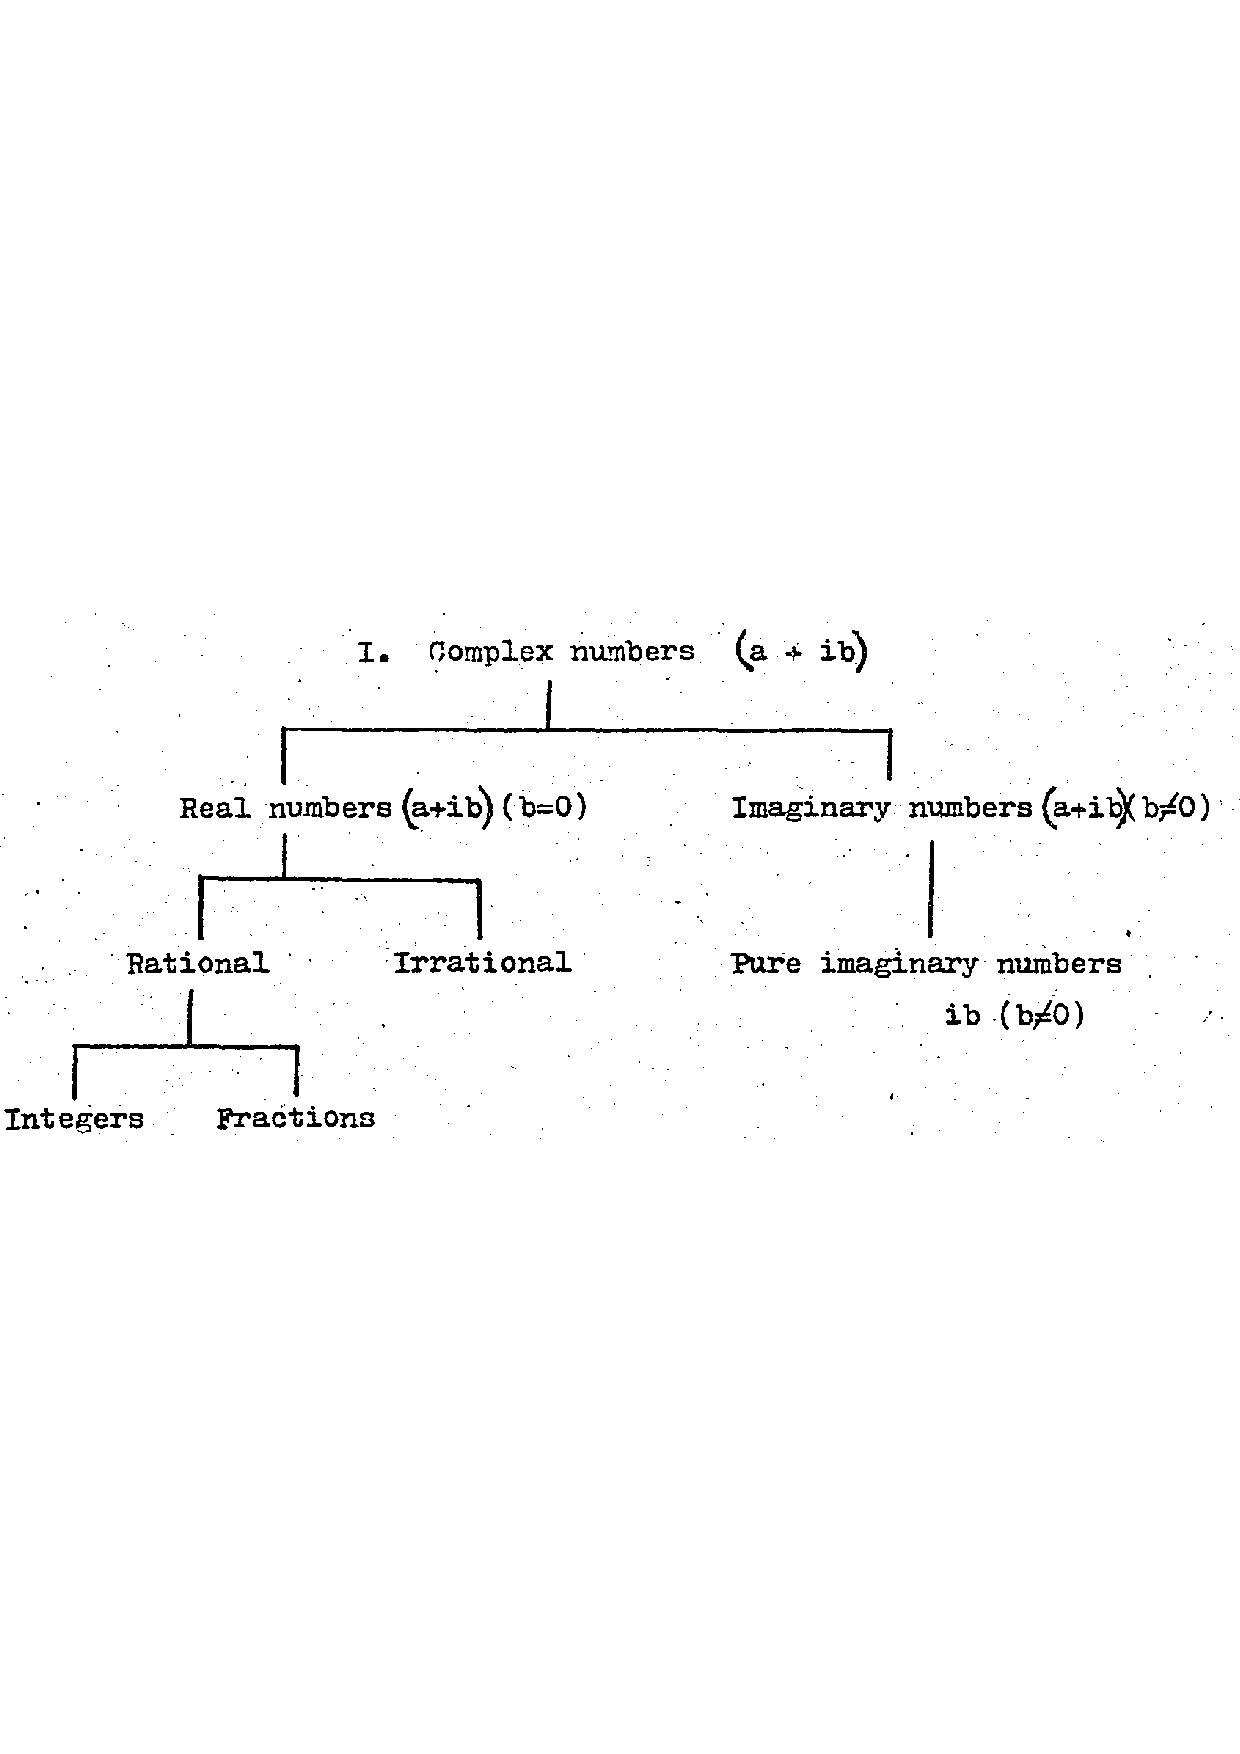
\includegraphics[width=0.9\textwidth]{images/SD-1-1p15A}
%	\caption{Classification of complex numbers}
%	\label{fig:classificationOfComplexNumbersA}
%\end{figure}

%\begin{center}
%\begin{tabular}{cc}
%\end{tabular}
%\end{center}

%\begin{exmp}
%\begin{hSolution}
%\end{hSolution}
%\end{exmp}

%\begin{hEnumerateAlpha}
%\end{hEnumerateAlpha}

%\begin{hEnumerateRoman}
%\end{hEnumerateRoman}

%$
%\begin{bmatrix}
%\end{bmatrix}
%$

%\frac{aaaa}{bbb}
%\frac{a_{n}}{b_{n}}
%\left( aaaa \right)
%\Longrightarrow

%\begin{multicols}{2}
%	bb
%\columnbreak
%	aa
%\end{multicols}
